\section{Large numbers of areas}

\setlength{\parindent}{0pt}

\subsection{Data augmentation}

XXX

\subsection{Distance-dependent dispersal function}

Minimize the number of parameters.
XXX

%setwd("/Users/mlandis/projects/RB_Biogeography_tutorial/")
\noindent \\ \impmark Open the RevBayes console

\begin{snugshade}
\begin{lstlisting}
$ revbayes
\end{lstlisting}
\end{snugshade}

First, we'll assign all our input files to {\tt String} variables.
\begin{snugshade}
\begin{lstlisting}
in_fp   <- "./data/"
data_fn <- "psychotria_range.nex"
area_fn <- "hawaii_dynamic.atlas.txt"
out_fp  <- "./output/"
out_str <- "bg_2rate"
\end{lstlisting}
\end{snugshade}

Then we'll create our range data, tree, and atlas objects

\begin{snugshade}
\begin{lstlisting}
data  <- readDiscreteCharacterData(in_fp + data_fn)
tree  <- readTrees(in_fp + data_fn)[1]
atlas <- readAtlas(in_fp + area_fn)
\end{lstlisting}
\end{snugshade}

Finally, we'll be using a few helper variables to create or move and monitor vectors
\begin{snugshade}
\begin{lstlisting}
mvi = 1
mni = 1
\end{lstlisting}
\end{snugshade}

\subsection{Creating the model}

Here, we will compose our rate matrix, {\bf Q}, parameterized by the transition rates, $\lambda$, and the distance dependent dispersal power parameter, $\beta$.

First, for $\lambda$, we will create a vector of two rates, where {\tt glr[1]} corresponds to the rate of area loss (local extinction) and {\tt glr[2]} corresponds to the rate of area gain (dispersal).
Each rate will be drawn from an exponential distribution with rate 10.0 (mean 0.1).
Because our tree is in units of millions of years, this means our prior expectation is that any given species undergoes one dispersal or extinction event per area per ten million years.

%setwd("/Users/mlandis/projects/RB_Biogeography_tutorial/")

Let's declare the distributions for these priors along with their MCMC moves

\begin{snugshade}
\begin{lstlisting}
for (i in 1:2) {
	glr[i]       ~ dnExponential(10.0)
	moves[mvi++] = mvScale(x=glr[i], lambda=0.5, tune=true, weight=5.0)
}
\end{lstlisting}
\end{snugshade}

These are then inserted into the rate matrix {\tt $q_area$}, which gives the average rate of area gain and loss per area.

\begin{snugshade}
\begin{lstlisting}
q_area := fnFreeBinary(glr)
\end{lstlisting}
\end{snugshade}

Next, we will create {\tt dp}, which determines the importance of geographical distance to dispersal.
Remember that values of $\beta$ far from zero means distance is important.
So, if we we assign a prior that pulls $\beta$ towards zero, then posterior values of $\beta$ far from zero indicate the range data are informative of the importance of distance to dispersal.
We'll use an exponential distribution with rate 10.0 (mean 0.1) as a prior for {\tt dp}.

\begin{snugshade}
\begin{lstlisting}
dp ~ dnExponential(10.0)
moves[mvi++] = mvScale(x=dp, lambda=0.5, tune=true, weight=5.0)
\end{lstlisting}
\end{snugshade}

We will also create a deterministic node to modify the rate of dispersal between areas by evaluating {\tt dp} and {\tt atlas}.
This node is determined by the function {\tt fnBiogeoGRM}, where GRM stands for ``geographical rate modifier'', and plays the role of the $\eta(\cdot)$ rate-modifier function mentioned earlier.
We will tell the {\tt fnBiogeoGRM} function to modify dispersal rates based on distances and whether or not the area exists during an epoch.

\begin{snugshade}
\begin{lstlisting}
grm := fnBiogeoGRM(atlas=atlas, distancePower=dp, useAvailable=true, useDistance=true)
\end{lstlisting}
\end{snugshade}

Now we need a deterministic node to represent the rate matrix, {\bf Q}.
To determine the value of this node, we'll use the function {\tt fnBiogeoDE} to assign our model parameters to transition rates as described in the introduction.
As input, we'll pass our gain and loss rates, {\tt glr}, and our geographical rate modifier, {\tt grm}.
In addition, we'll inform the function of the number of areas in our analysis and whether we will allow species to be absent in all areas (i.e. have the null range).

\begin{snugshade}
\begin{lstlisting}
q_range := fnBiogeoDE(gainLossRates=q_area, geoRateMod=grm, numAreas=4, forbidExtinction=true)
\end{lstlisting}
\end{snugshade}

To extract information for the frequencies of different cladogenic event types, we will create a Dirichlet-distributed stochastic node.
The simplex is over three events, subset sympatry (index 0), allopatry (index 1), and widespread sympatry (index 2), but not over narrow sympatry whose range size is one.
The prior parameter {\tt [1,1,0.1]} is known as a flat prior, meaning all event types are expected to occur at equal frequency.
If there is information in the data of a dominant cladogenic mode of range evolution, the posterior simplex values in {\tt csf} will reflect this.

\begin{snugshade}
\begin{lstlisting}
csf ~ dnDirichlet([1.,1.,0.5])
narrow_sympatry     := csf[1]
allopatry           := csf[2]
widespread_sympatry := csf[3]
moves[mvi++] = mvSimplexElementScale(csf, alpha=10.0, tune=true, weight=4.0)
\end{lstlisting}
\end{snugshade}

For the model's final node, we create the stochastic node for the continuous-time Markov chain (CTMC).
This node's distribution is {\tt dnPhyloDACTMC} where {\tt DA} indicates the CTMC uses data-augmentation to compute the likelihood rather than Felsenstein's pruning algorithm.
To create the distribution, we must pass it our {\tt tree} and {\tt Q} objects, but additionally inform the distribution that it will be using a biogeographic model, that it will introduce the simple cladogenic range evolution events described in \citet{ree08} ({\tt useCladogenesis=true}), and that it will assign zero probability to a transition away from the null range state.

\begin{snugshade}
\begin{lstlisting}
M ~ dnPhyloDACTMC(tree=tree, Q=q_range, C=csf, type="biogeo", forbidExtinction=true, useCladogenesis=true)
\end{lstlisting}
\end{snugshade}

In addition to proposing new model parameter values, we must also propose new data-augmented states and events to properly integrate over the space of possible range histories.
The major challenge to sampling character histories is ensuring the character histories are consistent with the observations at the tip of the tree.
The proposals in this tutorial use \citet{nielsen02}'s rejection sampling algorithm, with some modifications to account for cladogenic events and epoch-based rate matrices.

The basic idea is simple.
Each time a character history proposal is called, it selects a node at random from the tree.
Path history proposals ({\tt mvPathCHRS()}) propose a new character history for the lineage leading to that node.
Node history proposals ({\tt mvNodeCHRS()}) propose a new character history for the node and for the three lineages incident to that node.
The character history proposal also samples some number of areas to update, ranging from one to all of the areas.
Once the new character history is proposed, the likelihood of the model is evaluated and the MCMC accepts or rejects the new state according to e.g. the Metropolis-Hastings algorithm.

Because these {\tt Move} objects update the character histories stored in the data-augmented CTMC node, e.g. {\tt M},
they require access to a {\tt TimeTree} object to know which lineages are sisters and whether the lineages span various epochs, and a {\tt RateMap\_Biogeography} object to propose new character histories.
The {\tt lambda} argument gives what proportion of areas' character histories to update.
Here, if {\tt lambda=0.2}, then the proposal will redraw character histories for each area with probability 0.2 (in addition to one random area with probability 1).
Below, we use two moves of each type with {\tt lambda=0.2} and {\tt lambda=1.0} for partial and full character history updates, respectively.
Indicating {\tt type="biogeo"} informs the {\tt Move} object to be aware of special character history constraints, such as cladogenic events and forbidden null ranges.
The {\tt weight} parameter should be assigned a value proportional to the number of nodes in the analysis to ensure proper mixing.

Let's create the character history moves as follows: conservative character history updates for paths and nodes, with {\tt lambda=0.2}

\begin{snugshade}
\begin{lstlisting}
moves[mvi++] = mvCharacterHistory(ctmc=M, qmap=q_range, tree=tree, lambda=0.2, type="Biogeo", graph="node", proposal="rejection", weight=40.0)
moves[mvi++] = mvCharacterHistory(ctmc=M, qmap=q_range, tree=tree, lambda=0.2, type="Biogeo", graph="branch", proposal="rejection", weight=40.0)
\end{lstlisting}
\end{snugshade}

and the same proposals for more drastic character history updates, with {\tt lambda=1.0}

\begin{snugshade}
\begin{lstlisting}
moves[mvi++] = mvCharacterHistory(ctmc=M, qmap=q_range, tree=tree, lambda=1.0, type="Biogeo", graph="node", proposal="rejection", weight=10.0)
moves[mvi++] = mvCharacterHistory(ctmc=M, qmap=q_range, tree=tree, lambda=1.0, type="Biogeo", graph="branch", proposal="rejection", weight=10.0)
\end{lstlisting}
\end{snugshade}

So we may evaluate the graphical model's likelihood, we tell the CTMC to observe the {\tt data} object, which will prime the model with data-augmented character histories.
Now {\tt M} has a defined likelihood value.
\begin{snugshade}
\begin{lstlisting}
M.clamp(data)
M.lnProbability()
   -56.0288
\end{lstlisting}
\end{snugshade}

Finally, we encapsulate our graphical model into a {\tt Model} object, which can learn the model's structure and dependencies from any model parameter.
\begin{snugshade}
\begin{lstlisting}
my_model = model(M)
\end{lstlisting}
\end{snugshade}

First, we'll create monitors for our simple parameters

\begin{snugshade}
\begin{lstlisting}
monitors[mni++] = mnScreen(glr, dp, narrow_sympatry, allopatry, widespread_sympatry, printgen=10)
monitors[mni++] = mnFile(glr, dp, narrow_sympatry, allopatry, widespread_sympatry, filename=out_fp+params_fn, printgen=10)
\end{lstlisting}
\end{snugshade}

Like any parameter, we can sample the augmented range histories from the MCMC to approximate the posterior distribution of range histories.
This is statistically equivalent to generating ancestral state reconstructions from a posterior distribution via stochastic mapping.
We will extract these reconstructions using special monitors designed for the {\tt dnPhyloDACTMC} distribution.

Next, we will create {\tt Mntr\_CharacterHistoryNewickFile} objects to record the sampled character history states for each node in the tree.
This {\tt Monitor} has two {\tt style} options: {\tt counts} reports the number of gains and losses per branch in a tab-delimited Tracer-readable format;  {\tt events} reports richer information of what happens along a branch, anagenically and cladogenically, using an extended Newick format.
How to read these file formats will be discussed in more detail in Section \ref{sec:posterior}.

\begin{snugshade}
\begin{lstlisting}
monitors[mni++] = mnCharHistoryNewick(filename=fp+out_str+".events.txt", ctmc=M, tree=tree, printgen=100, style="events")
monitors[mni++] = mnCharHistoryNewick(filename=fp+out_str+".counts.txt", ctmc=M, tree=tree, printgen=100, style="counts")
\end{lstlisting}
\end{snugshade}

As our last monitor, the {\tt Mntr\_CharacterHistoryNhxFile} records character history values throughout the MCMC analysis, then stores some simple posterior summary statistics as a Nexus file.
These summary statistics could be computed from the previously mentioned {\tt Monitor} output files, but {\tt mnCharHistoryNhx} provides a simple way to produce Phylowood-compatible files.
We will also discuss this file's format in more detail later in the tutorial.

\begin{snugshade}
\begin{lstlisting}
monitors[mni++] = mnCharHistoryNhx(filename=fp+out_str+".nhx.txt", ctmc=M, tree=tree, atlas=atlas, samplegen=100, maxgen=25000, burnin=0.2)
\end{lstlisting}
\end{snugshade}

WE CAN REPLACE THIS USING WRITETREE->FIGTREE
Before we run the MCMC, we'd like to get the node index of the ancestor 
When analysing the output, we'll take some special interest in the branch for the most recent common ancestor of {\it P. kaduana} and {\it P. hatheway}.
We will identify this lineage by its index, 23, which is meaningful only for a fixed tree topology,
\begin{snugshade}
\begin{lstlisting}
> names = tree.names()
> names[15]
   P_kaduana_PuuKukuiAS
> names[16]
   P_hathewayi_1
> mrcaIndex(tree=tree,clade=clade(names[15],names[16]))
   23
\end{lstlisting}
\end{snugshade}


\subsection{Running an MCMC analysis}

Now all that's left is to configure and run our MCMC analysis.
For this, we create an {\tt Mcmc} object, which we give our {\tt Move} vector, our {\tt Monitor} vector, and our {\tt Model object}

\begin{snugshade}
\begin{lstlisting}
my_mcmc = mcmc(my_model, monitors, moves)
\end{lstlisting}
\end{snugshade}

MCMC typically requires some period of burn-in before it reaches stationarity, i.e. from a random starting point, it takes some time for the chain to produce valid samples from the posterior distribution.
By running {\tt burnin()}, we tell the {\tt Mcmc} object to propose and reject new states but {\it not} to record anything to file.
After burn-in is complete, we call {\tt run()}, where we begin recording valid posterior samples under our model.

\begin{snugshade}
\begin{lstlisting}
my_mcmc.run(generations=25000)
\end{lstlisting}
\end{snugshade}

Everything we've done is contained in the file {\tt biogeography\_DEC\_2rate.Rev}.
You can modify this file as you like then re-run the analysis by typing

\begin{snugshade}
\begin{lstlisting}
source("./scripts/biogeography_DEC_2rate.Rev")
\end{lstlisting}
\end{snugshade}


\subsection{Output}

\subsubsection{Sampled parameters from {\tt ScreenMonitor}}

\noindent \\ \impmark Open Tracer, select the fields for the posterior probability and area gain rate, {\tt glr[2]}, then click the Joint-Marginal tab.

\begin{figure}[H]
\centering
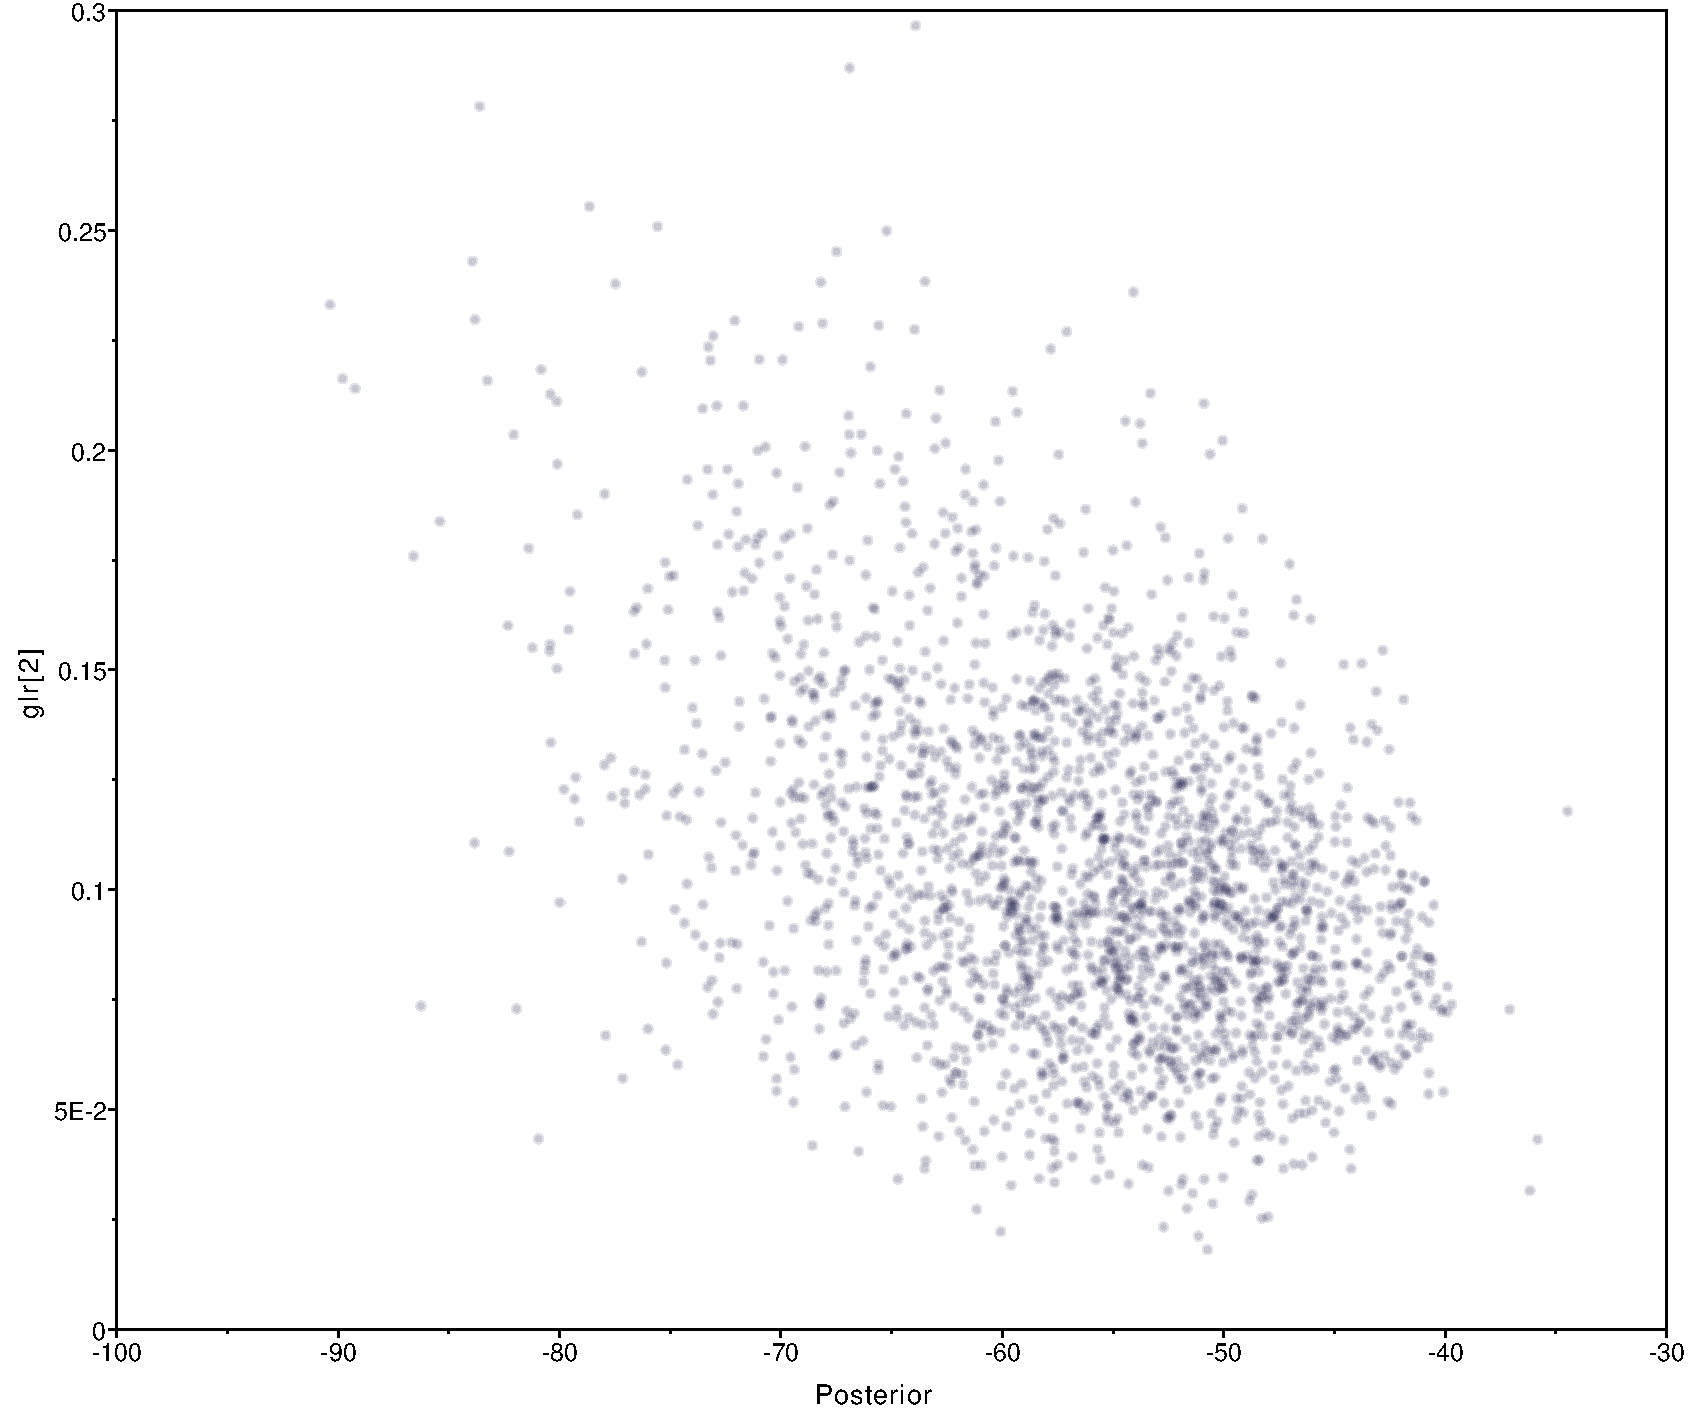
\includegraphics[width=3in]{figures/joint_rgain_posterior}
\caption{Joint-marginal distribution of posterior and area gain rate, $\lambda_1$.}
\end{figure}

Here, we see a strong negative correlation between the posterior probability and the area gain rate, which is expected.
Next, click the Estimates tab then select the three {\tt csf} parameters.

\begin{figure}[H]
\centering
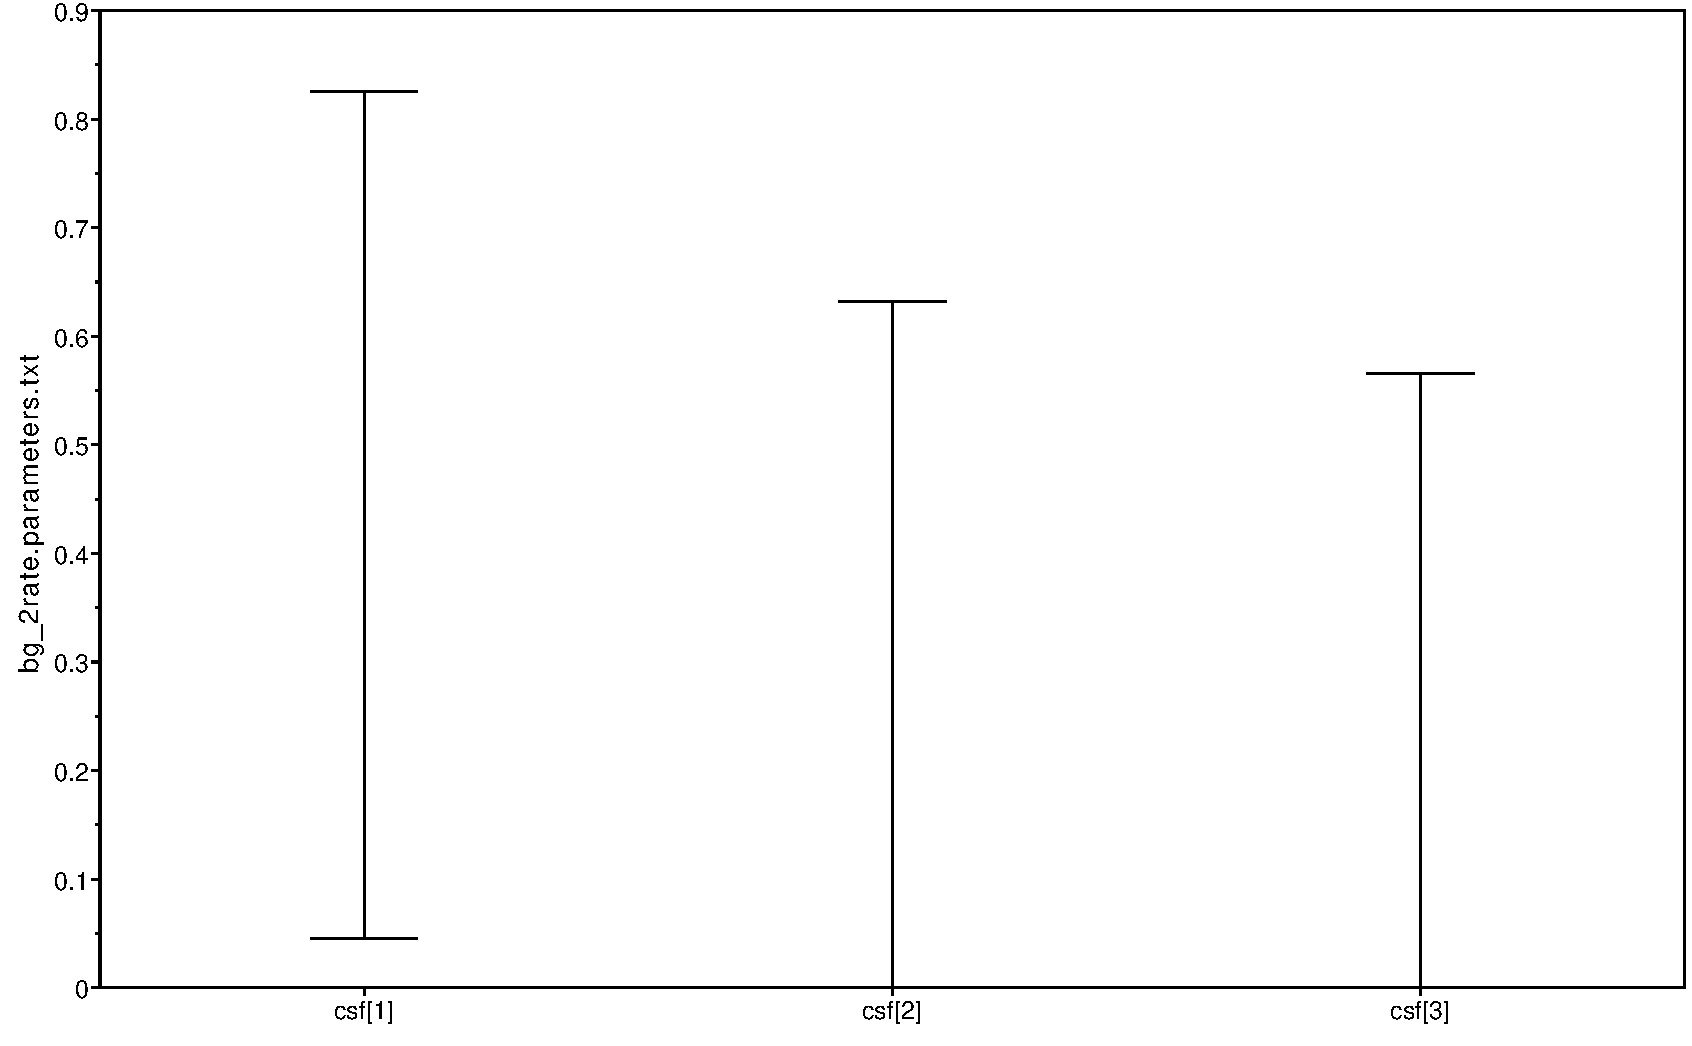
\includegraphics[width=3in]{figures/clado_freq_posterior}
\caption{Mean values for the cladogenic state frequency simplex, where {\tt csf[1]}, {\tt csf[2]}, and {\tt csf[3]} correspond to subset sympatry, allopatry, and wide sympatry whose mean posterior values are 0.45, 0.30, and 0.25, respectively.}
\end{figure}


\subsection{Biogeographic event counts from {\tt mnCharHistoryNewick}}

Recording stochastic mappings in a Tracer-compatible format requires some summarization.
This monitor generates a tab-delimited file where the number of events of each type for each branch is recorded.

\noindent \\ \impmark Open {\tt ./output/bg\_2rate.counts.txt} in a text editor.

\begin{framed}
\begin{lstlisting}%[basicstyle=\tiny \listingsfont, columns=texcl]
Iteration  Posterior  Likelihood    Prior	t_s0	t_s1	t_c0	t_c1	t_c2	t_c3	b0_s0	b0_s1	b0_c	...
0           -51.3307    -56.0288  4.69806	9	9	18	0	0	0	1	1	0	...	
10          -54.4257    -58.1568  3.73110	9	10	17	0	0	1	1	1	0	...
20          -58.0696    -62.0923  4.02274	11	9	15	2	1	0	2	1	1	...
30          -46.5049    -51.1197  4.61480	8	8	18	0	0	0	1	1	0	...
40          -42.8697    -46.4870  3.61735	7	7	18	0	0	0	1	1	0	...
50          -43.5319    -47.4659  3.93394	7	7	18	0	0	0	1	1	0	...
...
\end{lstlisting}
\end{framed}

For example, {\tt b2\_s1} gives the number of areas that are gained for the branch leading to the node indexed 2.
{\tt b2\_c} gives the cladogenic event type that gives rise to the node indexed 2, where narrow sympatry, subset sympatry, allopatry, and widespread sympatry are recorded as {\tt 0}, {\tt 1}, {\tt 2}, and {\tt 3}, respectively. The columns {\tt t\_s0} and {\tt t\_s1} give the sum of events over all branches. {\tt t\_c0}, {\tt t\_c1}, and {\tt t\_c2} give the total number of narrow sympatric, subset sympatric, allopatric, and widespread sympatric cladogenic events over the entire tree.

Because the expected number of gain events should be proportional to the area gain rate, we expect to see the same negative correlation between posterior probability and number of events as we did with the posterior and rate in the {\tt parameters.txt} file.

Open Tracer, select the fields for the posterior probability and the number of gained areas over the tree, {\tt t1}, then click the Joint-Marginal tab.

\begin{figure}[H]
\centering
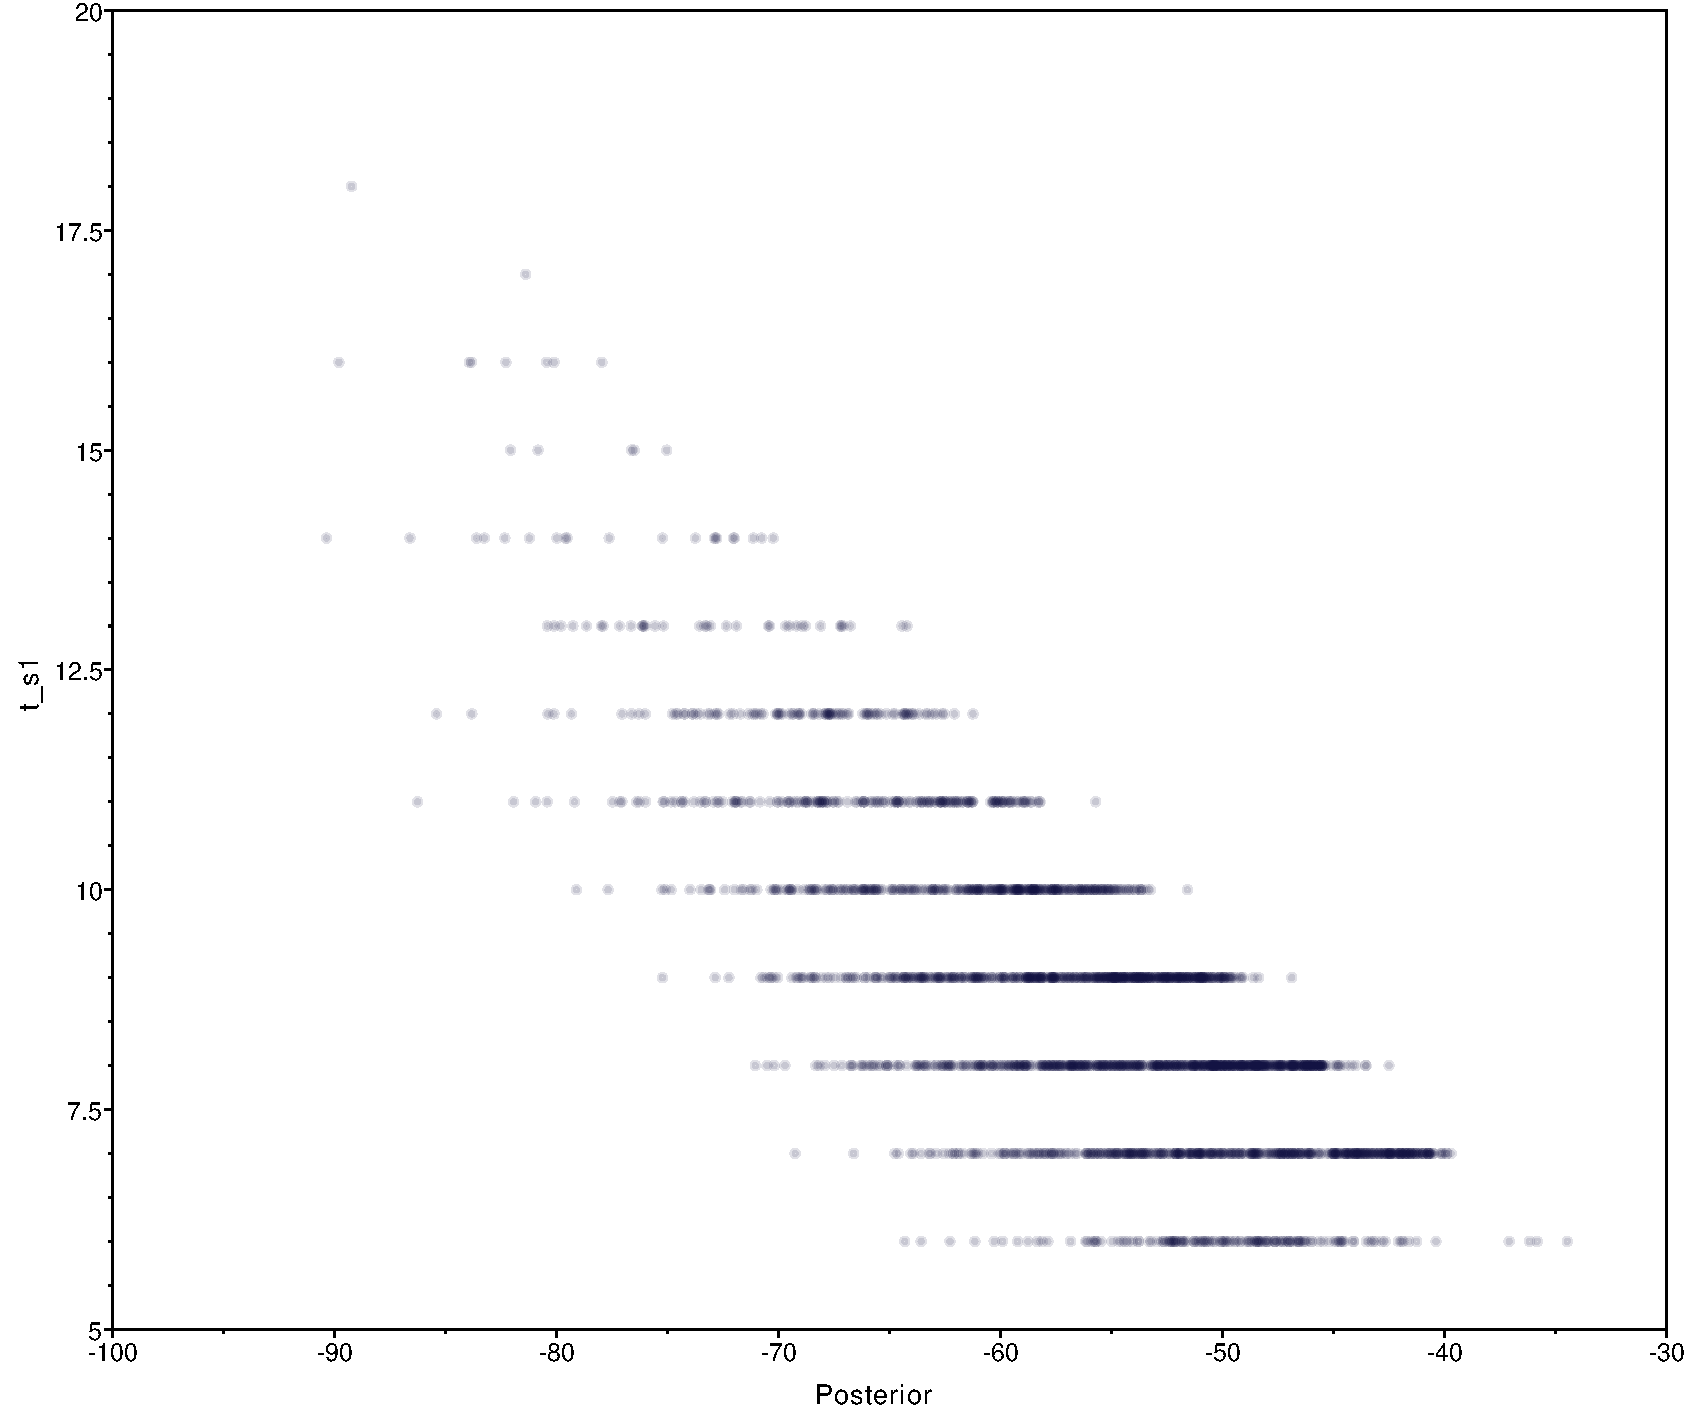
\includegraphics[width=3in]{figures/joint_ngain_posterior}
\caption{Joint-marginal distribution of posterior and number dispersal events summed over the tree.}
\end{figure}

One interesting facet of this output is there are never fewer than six events.
In fact, since we assume a stratified geography and that only one event may occur per instant, it is impossible to describe the data we see at the tips with fewer than six gain events.
That is, six gain events is part of the maximum parsimony solution.

\subsection{Biogeographic event histories from {\tt mnCharHistoryNewick}}

For more detailed data exploration, this analysis also provides annotated Newick strings with the complete character mappings for the tree.

\noindent \\ \impmark Open {\tt ./output/bg\_2rate.events.txt} in a text editor.

\begin{framed}
\begin{lstlisting}%[basicstyle=\tiny \listingsfont, columns=texcl]
Iteration  Posterior  Likelihood  Prior  Tree
Iteration	Posterior	Likelihood	Prior	Tree
0	-51.3307	-56.0288	4.69806	((((((((P_hawaiiensis_WaikamoiL1[&index=18;nd=0010;pa=0010;ev={}]:0.96 ...
10	-54.4257	-58.1568	3.7311	((((((((P_hawaiiensis_WaikamoiL1[&index=18;nd=0010;pa=0010;ev={}]:0.96 ...
20	-58.0696	-62.0923	4.02274	((((((((P_hawaiiensis_WaikamoiL1[&index=18;nd=0010;pa=0010;ev={}]:0.96 ...
30	-46.5049	-51.1197	4.6148	((((((((P_hawaiiensis_WaikamoiL1[&index=18;nd=0010;pa=0010;ev={}]:0.96 ...
40	-42.8697	-46.4870	3.61735	((((((((P_hawaiiensis_WaikamoiL1[&index=18;nd=0010;pa=0010;ev={}]:0.96 ...
50	-43.5319	-47.4659	3.93394	((((((((P_hawaiiensis_WaikamoiL1[&index=18;nd=0010;pa=0010;ev={}]:0.96 ...

...
\end{lstlisting}
\end{framed}

Each iteration records the data-augmented character history (stochastic mapping) using metadata labels, which, for an internal node, looks like

\begin{snugshade}
\begin{lstlisting}
[&index=23;nd=0110;pa=0010;ch0=0010;ch1=0110;cs=s;bn=16;ev={{t:0.2513,a:1.1195,s:1,i:1}}
\end{lstlisting}
\end{snugshade}

{\tt index=23} indicates this branch leads to the node indexed 23.
The branch began in the ancestral state {\tt pa=0100} and terminated in the state {\tt nd=0110}.
Since this node is not a tip node, it represents a speciation event, so the daughter ranges are also given, {\tt ch0=0010} and {\tt ch1=0110}.
The cladogenic state for this speciation event was subset sympatric, {\tt cs=s}, rather than sympatric (wide or narrow; {\tt w} or  {\tt n}) or allopatric ({\tt a}).
Anagenic dispersal and extinction events occurring along the lineage leading to node 19 are recorded in {\tt events}, where each event has a time (relative to the absolute branch length), absolute age, state (into), and character index ({\tt t}, {\tt a}, {\tt s}, {\tt i}, resp.).
For this posterior sample of the character history for the branch leading to node 22, the species range expanded into Oahu at age 1.1195.

To manipulate this data format, we'll use Python scripts. Below are a few examples of interesting posterior features.

\noindent \\ \impmark  Open a Python console and read in the events.

\begin{snugshade}
\begin{lstlisting}
> cd scripts
> python27

...

>>> from bg_parse import *
>>> dd=get_events(fn="../output/bg_2rate.events")
\end{lstlisting}
\end{snugshade}

By default, {\tt get\_events()} extracts a dictionary where each node index maps to a branch's character history as reported in {\tt ./input/bg\_2rate.events.txt}. 
Each branch is a dictionary whose keys are various parts of the MCMC state and whose values the MCMC samples.
\begin{snugshade}
\begin{lstlisting}
>>> dd[23].keys()
['ch1', 'iteration', 'bn', 'nd', 'ch0', 'prior', 'posterior', 'cs', 'ev', 'likelihood']
>>> dd[23]['posterior'][0:5]
[-48.6952, -60.1832, -53.2286, -57.5778, -53.4633]
\end{lstlisting}
\end{snugshade}

To get the $n=1$ highest-valued sample for a branch by its posterior value
\begin{snugshade}
\begin{lstlisting}
>>> get_best(dd[23],n=1,p='posterior')
{'prior': [4.48225], 'iteration': [14890], 'bn': [22], 'nd': [[0, 1, 1, 0]], 'ch0': [[0, 1, 1, 0]], 'ch1': [[0, 0, 1, 0]], 'posterior': [-34.7139], 'pa': [[0, 1, 0, 0]], 'cs': ['subset_sympatry'], 'ev': [[{'age': 1.5637, 'state': 1, 'idx': 2, 'time': 0.8611}]], 'likelihood': [-39.1962]}
\end{lstlisting}
\end{snugshade}

To get the probability that area $i$ and area $j$ are both part of the species range as the branch for node 23 terminates, just before the speciation event
\begin{snugshade}
\begin{lstlisting}
>>> get_area_pair(dd[23])
[[0.0816, 0.0188, 0.0628, 0.0000],
 [0.0188, 0.7081, 0.4390, 0.0000],
 [0.0628, 0.4390, 0.7141, 0.0000],
 [0.0000, 0.0000, 0.0000, 0.0000]]
\end{lstlisting}
\end{snugshade}
showing area 3 was occupied nearly with probability 0.71 and both areas 2 and 3 were occupied with probability 0.44.
Note, Hawaii was submerged until approximately 0.5 million years ago, and thus the probability of being in that area is 0.0.

If the range is size one during a speciation event, the cladogenic event state is always narrow sympatric, {\tt `narrow\_sympatry'}.
But given the opportunity for non-sympatric events, i.e. that the range is larger than size one, we can get the probability of cladogenic state using
For the probability for cladogenic event state given the range was larger than size one
\begin{snugshade}
\begin{lstlisting}
>>> get_clado_state(dd[23])
{'allopatry': 0.0224, 'subset_sympatry': 0.1463, 'widespread_sympatry': 0.3183, 'narrow_sympatry': 0.5130}
>>> get_clado_state(dd[23],minSize=2)
{'allopatry': 0.0460, 'subset_sympatry': 0.3005, 'widespread_sympatry': 0.6535, 'narrow_sympatry': 0.0000}
>>> get_clado_state(get_best(dd[23],n=100),minSize=2)
{'allopatry': 0.1290, 'subset_sympatry': 0.6774, 'widespread_sympatry': 0.1936, 'narrow_sympatry': 0.0000}
\end{lstlisting}
\end{snugshade}

Depending on your question, different aspects of the posterior cladogenic state will interest you.
Narrow sympatry is the favored ancestral state, but wide sympatry is favored for ranges of size $n>1$.
However, when we look at the 100 most probable samples, subset sympatry becomes most favored.

More script functions are found in {\tt ./scripts/bg\_parse.py}.

\subsection{New Hampshire extended format file (\texttt{./output/bg\_2rate.nhx})}

Because this data is very high-dimensional, we'll use an external data exploration tool to look at range evolution.

This file summarizes the input and output from a BayArea analysis using NEXUS format containing a New Hampshire eXtended (NHX) tree string.
NHX allows you to annotate nodes in a Newick string with meta-information, which BayArea uses to report the probabilities in the \texttt{my\_run.area\_probs.txt} file.
The \texttt{geo} block gives the geographical latitudes and longitudes for the areas in the order they are reported as probabilities.
Like the \texttt{my\_run.area\_probs.txt} file, this file is not written until the analysis is complete.
This annotation is used for the two visualization programs covered in the next section, Phylowood and BayArea-Fig.
The anatomy of the Phylowood and BayArea-Fig settings blocks will also be explained there.

\section{Visualization}

Here we'll explore two options for visualizing ancestral range reconstructions.
I'll walk you through some of the basic functionality, but feel free to play around as you like.

\subsection{Phylowood}

Phylowood generates interactive animations to explore biogeographic reconstructions.

\noindent \\ \impmark Open \texttt{http://mlandis.github.io/phylowood}.

\noindent \\ \impmark Drag and drop \texttt{./output/bg\_2rate.nhx.txt} into the text field.

\begin{figure}[H]
\centering
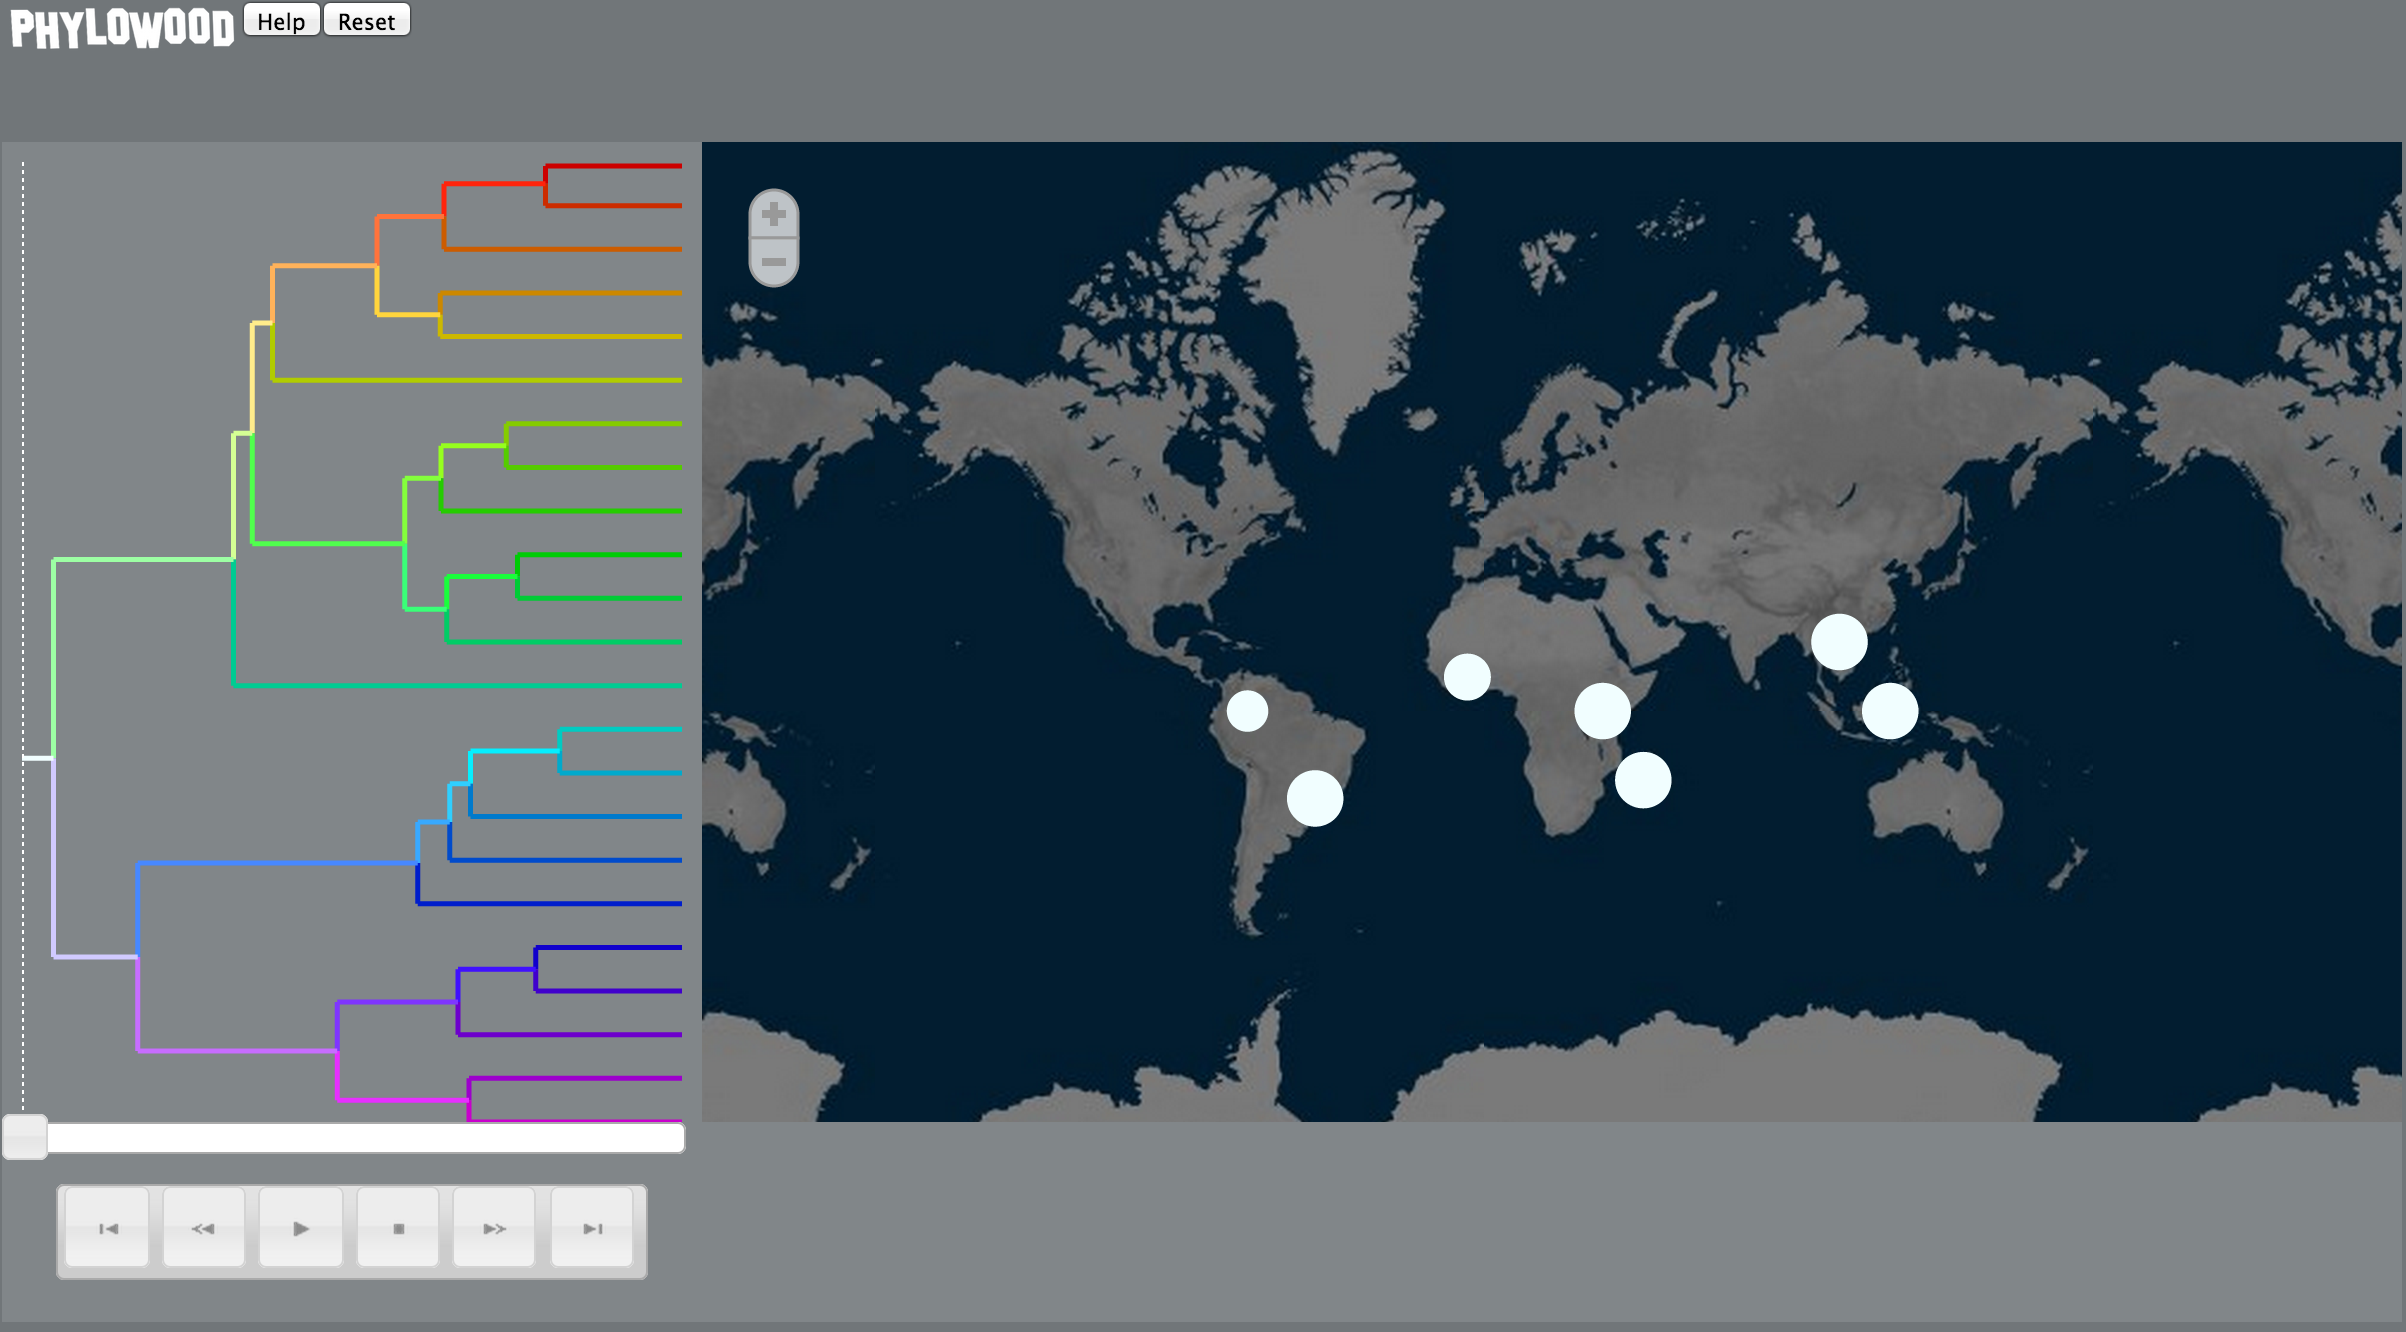
\includegraphics[width=4in]{figures/phw_mrca}
\caption{Phylowood frame showing posterior ancestral range of root node.}
\end{figure}

\noindent \\ \impmark Click the Play button to view the animation. \\

There are three control panels to help you filter data: the media panel, the map panel, and the phylogeny panel.
The media buttons correspond to Beginning, Slow/Rewind, Play, Stop, Fast Forward, Ending (from left to right).
The animation will play the timeframe corresponding to the slider.

\noindent \\ \impmark Drag the slider to the right (the present).

\begin{figure}[H]
\centering
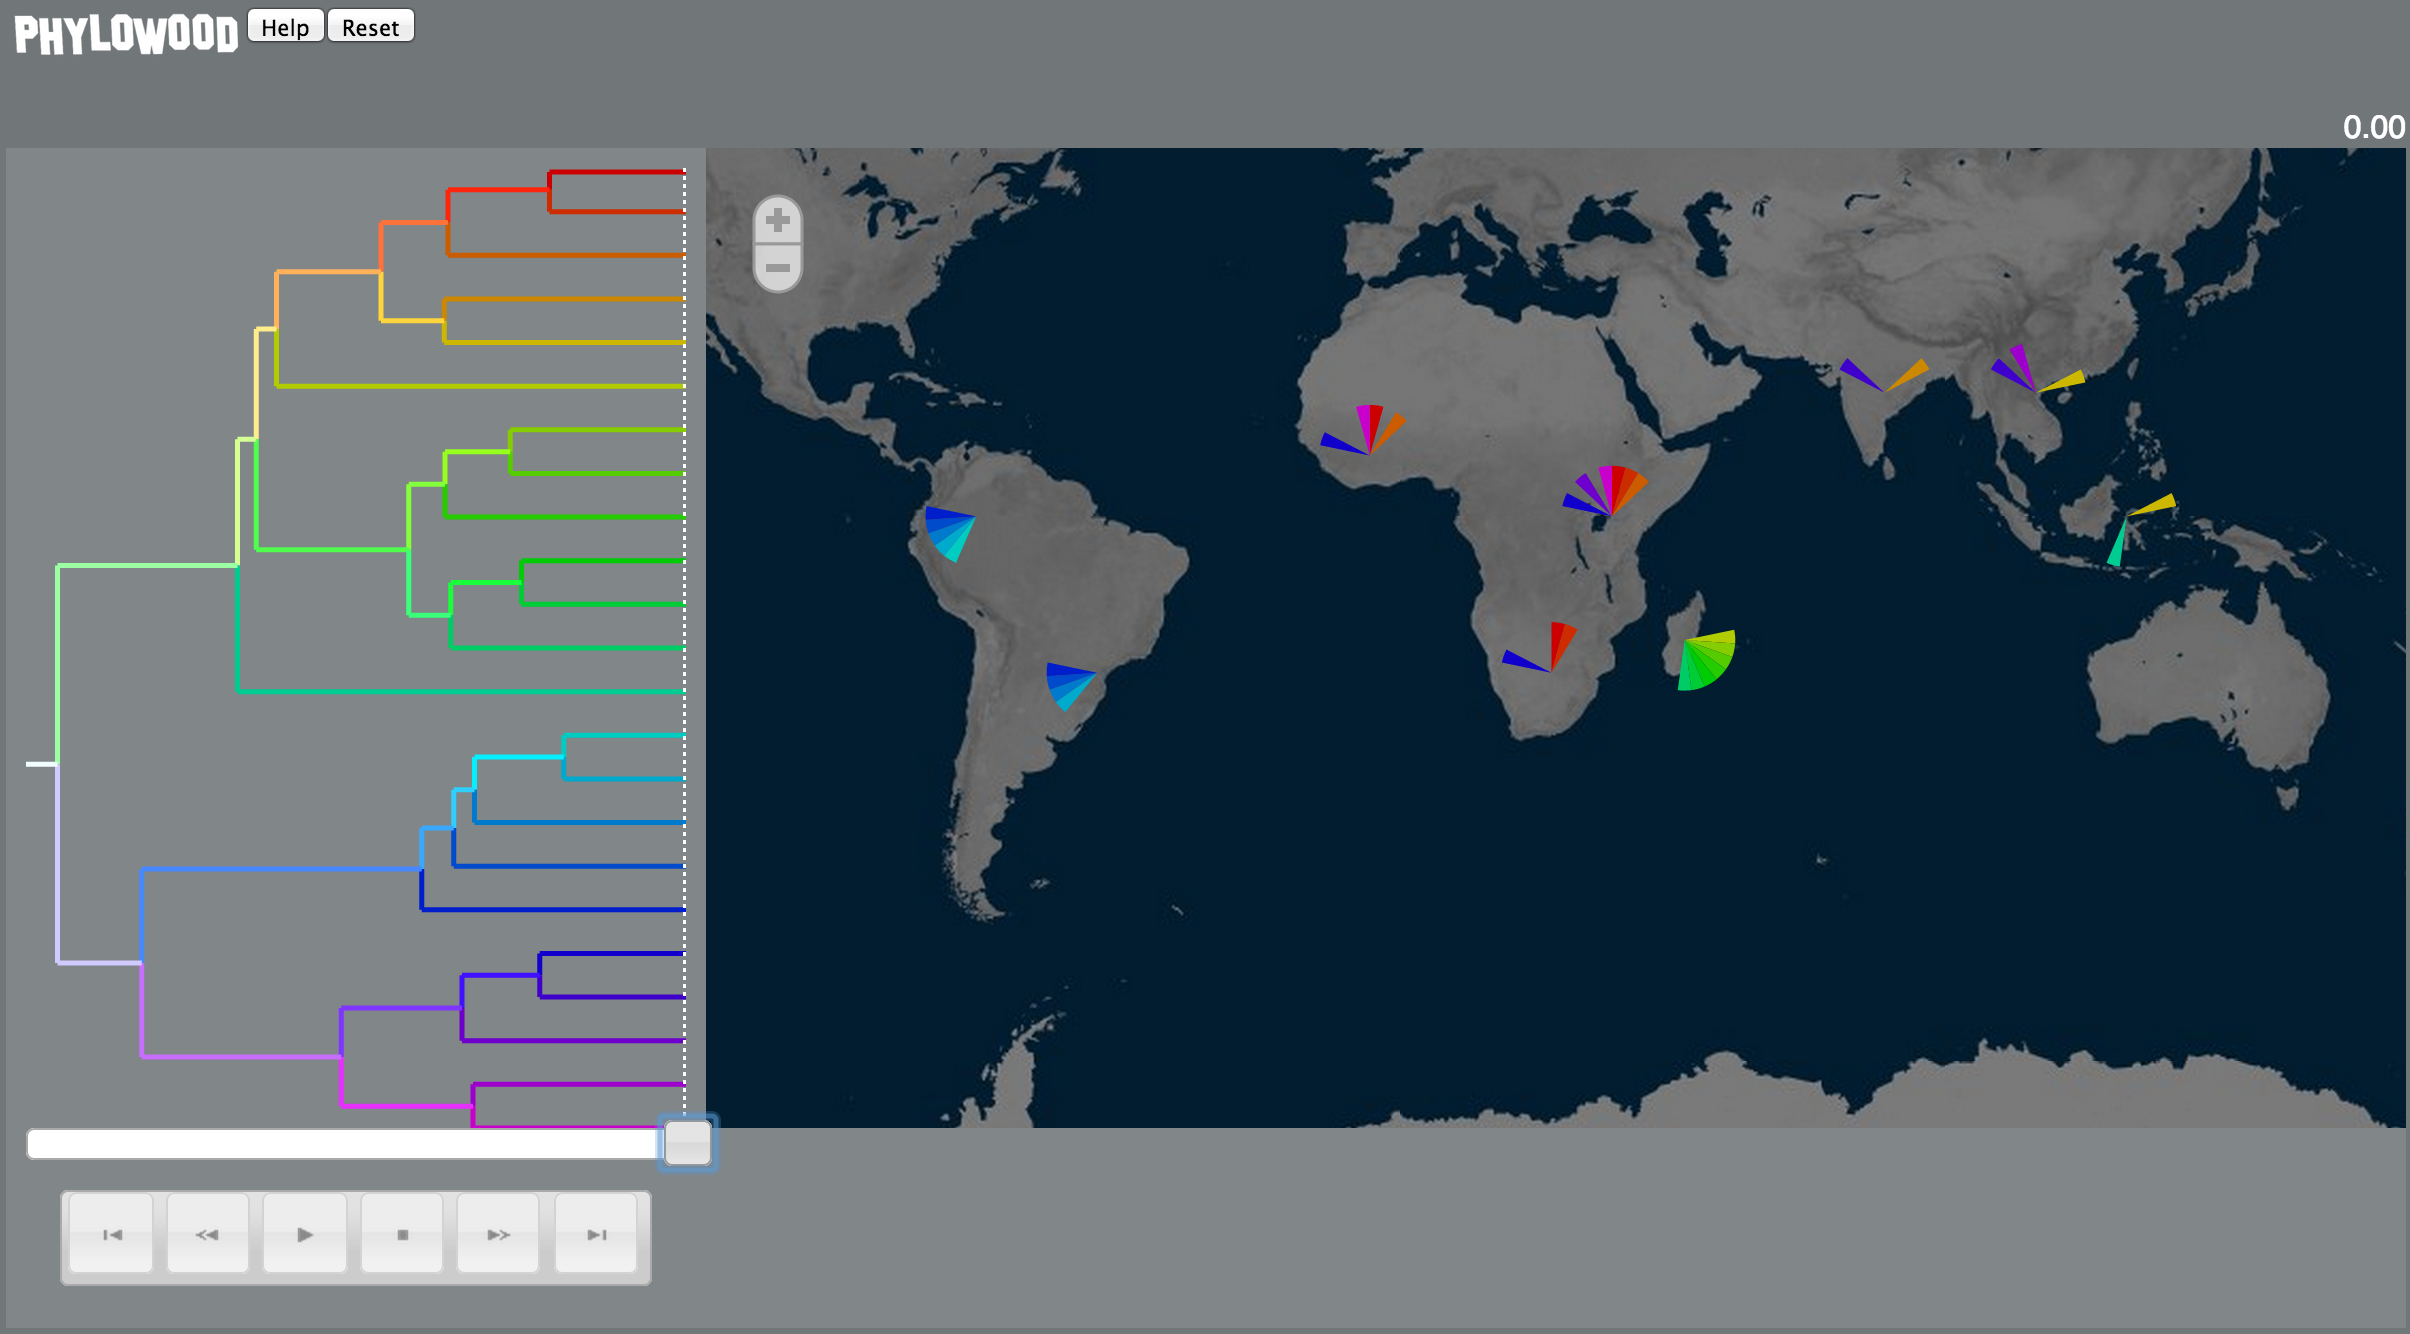
\includegraphics[width=4in]{figures/phw_all}
\caption{Phylowood frame showing distribution of extant taxon ranges.}
\end{figure}

\noindent \\ \impmark Pan and zoom around the map.\\

Marker colors correspond to the phylogenetic lineages in the phylogeny panel.
Markers are split into slices and (loosely) sorted phylogenetically, so nearby slices are generally closely related.
At divergence events, a marker's radius is proportional to the marginal posterior probability the node was present in the area at that time.
Between divergence events, marker's radius is simply an interpolation of the values at the two endpoints.
Some information about geological constraints and cladogenic events is lost.

\noindent \\ \impmark Mouseover an area to learn which lineage it belongs to and its presence probability. \\

Since it's difficult to see how specific clades evolve with so many taxa, Phylowood offers two ways to filter taxa from the animation.
We call the set of a lineage, all its ancestral lineages towards the root, and all descendant lineages a phylogenetic heritage.
The root's heritage is the entire clade.
A leaf node's heritage is a path from the tip to the root.

\noindent \\ \impmark Mouseover a lineage to temporarily highlight the lineage's heritage. Remove the mouseover to remove the highlight effect. \\

The highlight effect is temporary and quickly allows you to single out lineages of interest during animation.
Phylowood also offers a masking effect that persists until an unmask command is issued.

\noindent \\ \impmark Double-click the white root branch to mask the root node's heritage (all lineages). Single click a lineage to unmask that lineage's heritage. \\

\begin{figure}[H]
\centering
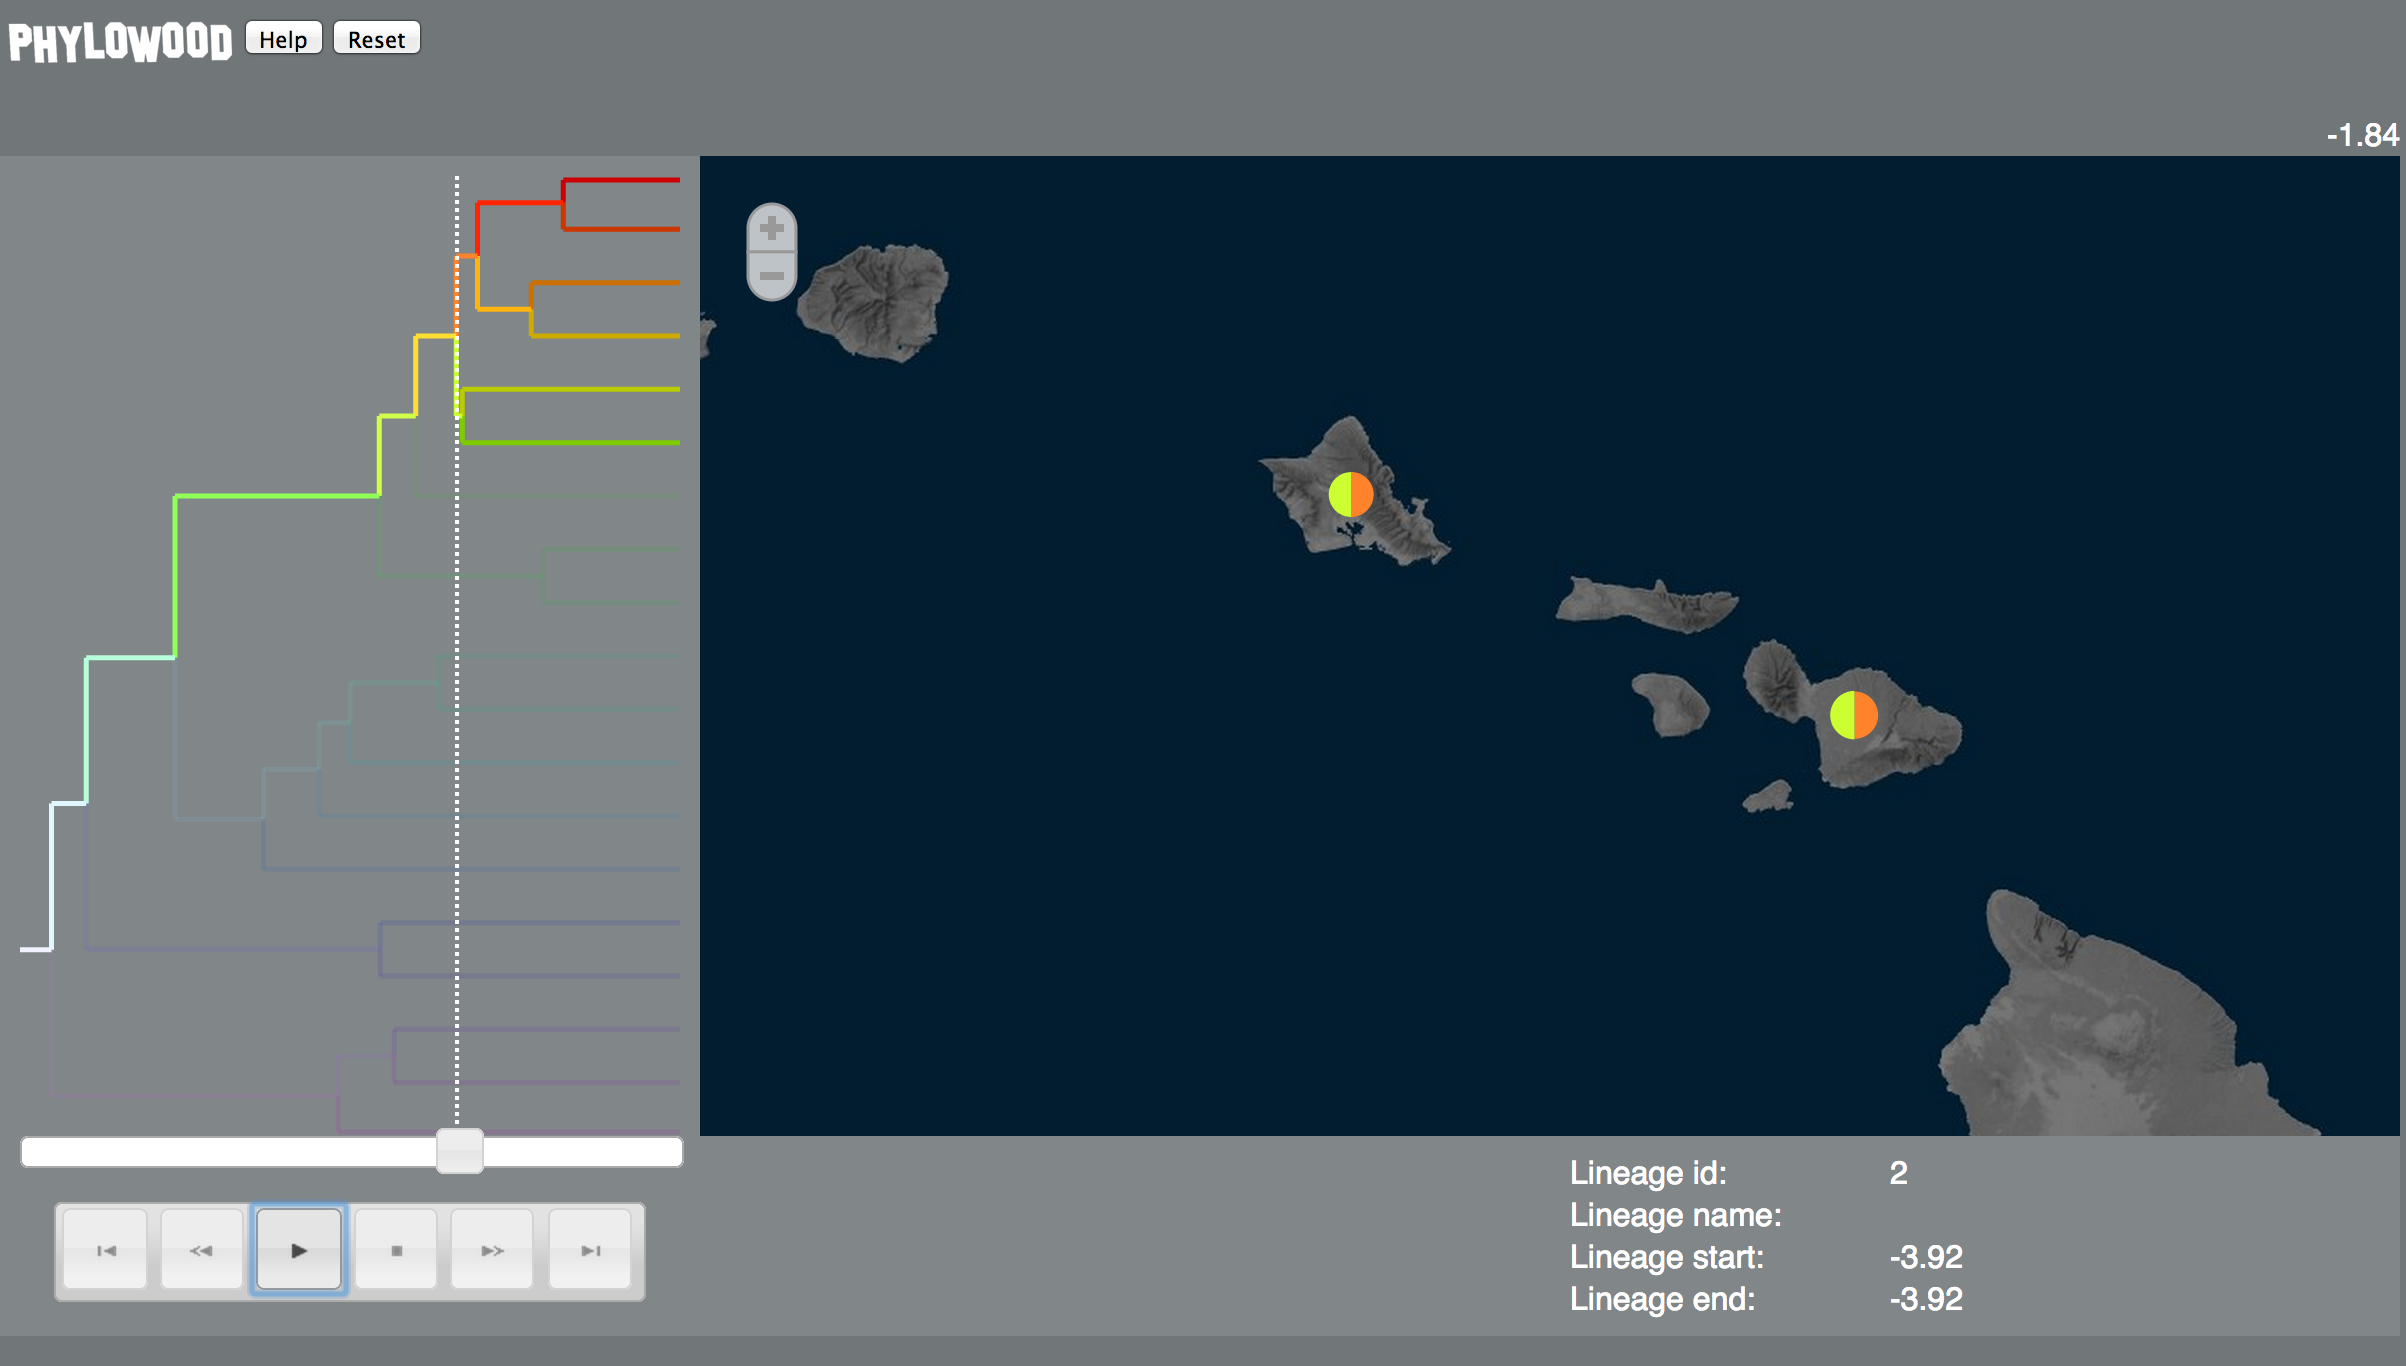
\includegraphics[width=4in]{figures/phw_br23}
\caption{Phylowood frame highlighting the posterior range for the most recent common ancestor of {\it P. mauiensis} and {\it P. hawaiiensis}.}
\end{figure}

Now that the masking effects are in place, you're free to interact with other map components.
In addition, the area of marker sizes is only distributed among unmasked lineages.

\noindent \\ \impmark Visit \texttt{https://github.com/mlandis/phylowood/wiki} to learn more about Phylowood.



%%%%%%%%%%%% GRAVEYARD %%%%%%%%%%%%%%%



%%\subsection{Model selection using Bayes factors}
%%
%%Bayes factors (BFs) are used to select which of two models better describes the observed data, $\mathbf{X}_{obs}$, and are computed as the ratio of marginal likelihoods for those two models.
%%One might prefer to analytically compute the marginal likelihood, but it's the same intractable quantity we intentionally avoid computing when using MCMC in a Bayesian context.
%%Instead, we must estimate the marginal likelihood from our posterior distribution samples.
%%Here, we will use thermodynamic integration \citep{lartillot06} and stepping-stone approximation \citep{xie10}.
%%The exact details of these techniques will not be covered here, but there is an important practical point to mention: both methods rely on computing a number of ``power posterior'' distributions.
%%Computing more power posteriors increases the marginal likelihood estimator's accuracy at the cost of computational time.
%%
%%Moving on, we'll compute the Bayes factor to compare a simple one-rate model, which asserts the rate of area gain and loss are always equal, to a two-rate model which allows these rates to vary independently.
%%Rather than specifying the model manually, we will load (source) the model definition from a file then enter the commands to compute its marginal likelihood.
%%For faster results, we will use two separate RevBayes sessions, one for each model.
%%For each session, the power posterior analysis run for 1000 generations during burn-in then 1000 generations per each of 30 power posterior categories.
%%
%%First session:
%%\begin{snugshade}
%%\begin{lstlisting}
%%RevBayes > source("./scripts/biogeography_DEC_1rate.Rev")
%%RevBayes > pp_fn <- out_fp + out_str + ".pp.txt"
%%RevBayes > pow_p <- powerPosterior(my_model, moves, pp_fn, cats=30) 
%%RevBayes > pow_p.burnin(generations=1000,tuningInterval=100)
%%RevBayes > pow_p.run(generations=5000)
%%\end{lstlisting}
%%\end{snugshade}
%%
%%Second session:
%%\begin{snugshade}
%%\begin{lstlisting}
%%RevBayes > source("./scripts/biogeography_DEC_2rate.Rev")
%%RevBayes > pp_fn <- out_fp + out_str + ".pp.txt"
%%RevBayes > pow_p <- powerPosterior(my_model, moves, pp_fn, cats=30) 
%%RevBayes > pow_p.burnin(generations=1000,tuningInterval=100)
%%RevBayes > pow_p.run(generations=5000)  
%%\end{lstlisting}
%%\end{snugshade}
%%
%%Each power posterior analysis will write their contents to the file given in {\tt pp\_fn}.
%%These files are {\tt bg\_1rate.pp.txt} and {\tt bg\_2rate.pp.txt} for the simple and complex models, respectively.
%%This may take a few minutes.
%%When complete, the power posterior files may then be used to compute marginal likelihoods.
%%For example, from the RevBayes session analyzing the simple one-rate model
%%
%%\begin{snugshade}
%%\begin{lstlisting}
%%RevBayes > ss <- steppingStoneSampler(file=pp_fn)
%%RevBayes > ss.marginal() 
%%RevBayes > ps <- pathSampler(file=pp_fn)
%%RevBayes > ps.marginal() 
%%\end{lstlisting}
%%\end{snugshade}
%
%For a given model, the path sampling and stepping stone sampling methods should produce similar marginal likelihood estimates.
%Values should be within one log likelihood unit of one another.
%If the values are extremely different, this may indicate {\tt powerPosterior} should be re-run with a larger number of {\tt cats}.
%We chose {\tt cats=30} which should suffice, and we see no problem.
%Then from the complex two-rate model RevBayes session using the same commands as above.
%Finally, we can compute the Bayes factor, which is simply the ratio of marginal likelihoods.
%
%\begin{snugshade}
%\begin{lstlisting}
%RevBayes > exp(-51.7202)/exp(-52.3158)
%   1.81412
%\end{lstlisting}
%\end{snugshade}
%
%A value of one would mean both models had equal marginal likelihoods.
%A value less than one would indicate the first model, the simple model, had a larger marginal likelihood, and was therefore favored by model testing.
%But that's not the case, the value is greater than one, and the complex two-rate model is favored.
%Similar to frequentist interpretations of significance for p-values, there is no universal and objective criterion of significance with Bayes factors, but most would agree a factor of 1.8 (or 1.0/1.8) indicates weak support for one model over the other.



%The {\tt mnScreen} monitor reports model parameter values to the screen, where each row corresponds to the current accepted MCMC state, and each column reports some model feature, such as the model likelihood or a parameter value.
%Every 20 iterations, this monitor re-prints the column headers.
%
%\begin{snugshade}
%%\begin{lstlisting}[basicstyle=\tiny \listingsfont, columns=texcl]
%\begin{lstlisting}%[basicstyle=\tiny \listingsfont]
%RevBayes > my_mcmc.run(generations=25000)
%
%Running MCMC simulation for 25000 iterations
%The simulator uses 8 different moves in a random
%move schedule with 241 moves per iteration
%
%Iteration   |   Posterior  |          dp  |      glr[1]  |      glr[2]  |      csf[1]  |      csf[2]  |      csf[3]
%-------------------------------------------------------------------------------------------------------------------
%0           |    -51.3307  |   0.0570518  |    0.175137  |   0.0580957  |    0.330891  |    0.255308  |    0.413801
%10          |    -54.4257  |   0.0416423  |    0.166936  |    0.178402  |   0.0549136  |    0.148854  |    0.796233
%20          |    -58.0696  |   0.0991853  |    0.136495  |    0.122135  |    0.308418  |    0.448892  |    0.242689
%30          |    -46.5049  |     0.10676  |   0.0958918  |   0.0959592  |    0.543837  |    0.363871  |   0.0922922
%40          |    -42.8697  |    0.173549  |    0.158565  |   0.0662419  |    0.569416  |    0.126439  |    0.304145
%50          |    -43.5319  |    0.117868  |    0.196497  |   0.0523307  |    0.440269  |    0.257171  |     0.30256
%
%...
%\end{lstlisting}
%\end{snugshade}
%
%For the complex 2-rate model, our model parameters are {\tt dp}, the distance power parameter, and the rates of area loss and gain, {\tt glr[1]} and {\tt glr[2]}, respectively, and the frequencies for subset sympatry, allopatry, and widespread sympatry {\tt csf[1]}, {\tt csf[2]}, and {\tt csf[3]}, respectively. 
%If you notice the value of some parameter is rarely updated from iteration to iteration, the MCMC is probably mixing poorly therefore it's not generating samples from the posterior distribution (the MCMC's stationary distribution).
%In this case, you may want to re-run the analysis with different arguments for the {\tt Move} object assigned to that parameter.
%
%\subsection{Sampled parameters from {\tt ModelMonitor}}
%
%This tab-delimited file contains parameter samples from the posterior distribution.
%As with the {\tt ScreenMonitor}, columns are model or parameter values and rows are MCMC cycles.
%
%\begin{framed}
%\begin{lstlisting}%[basicstyle=\tiny \listingsfont, columns=texcl]
%Iteration  Posterior  Likelihood    Prior  glr[1]  glr[2]  dp  csf[1]  csf[2]  csf[3]
%0           -51.3307    -56.0288  4.69806  0.175137  0.0580957  0.057051  0.330891  0.255308  0.413801
%10          -54.4257    -58.1568  3.73110  0.166936  0.1784020  0.041642  0.054913  0.148854  0.796233
%20          -58.0696    -62.0923  4.02274  0.136495  0.1221350  0.099185  0.308418  0.448892  0.242689
%30          -46.5049    -51.1197  4.61480  0.095891  0.0959592  0.106760  0.543837  0.363871  0.092292
%40          -42.8697    -46.4870  3.61735  0.158565  0.0662419  0.173549  0.569416  0.126439  0.304145
%50          -43.5319    -47.4659  3.93394  0.196497  0.0523307  0.117868  0.440269  0.257171  0.302560
%
%...
%\end{lstlisting}
%\end{framed}
